\chapter{Background}
\label{chap:background}

In this chapter we are going to explain the most important concepts of the
upcoming 5G standard, talking about the Virtual Network Functions (VNFs), the
Network Slice (NS) concept and how first experiments with these new innovations
already begun. Finally we are going to briefly introduce and explain the
technologies involved and their role.

\section{The 5G connectivity standard}

\begin{figure}[t]
  \centering
  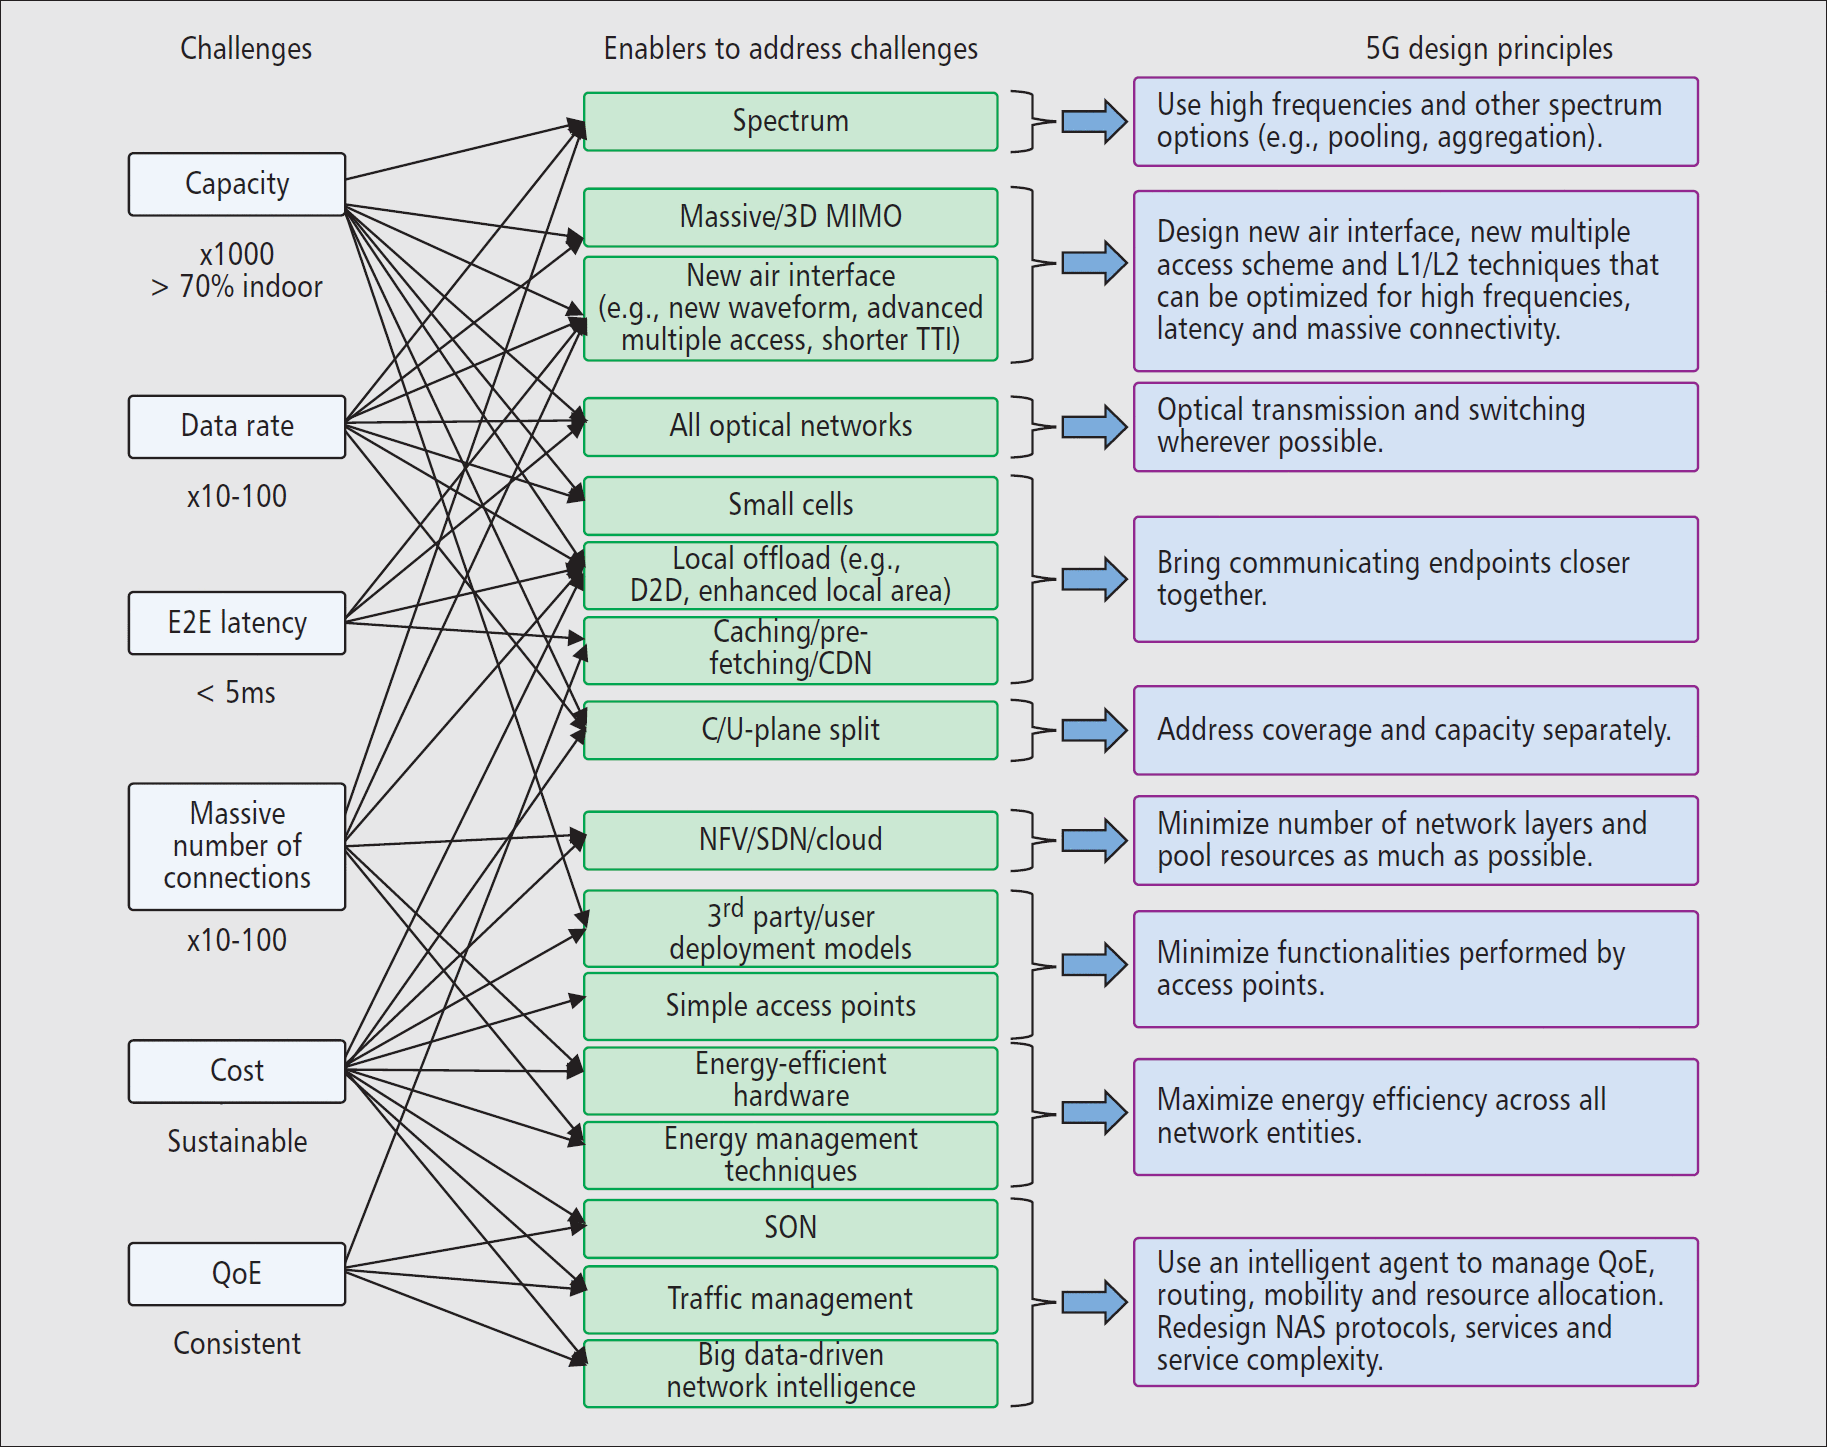
\includegraphics[scale=0.8]{5GEnablers}
  \caption[5G enablers]{5G enablers. It is possible to see that the NFV/SDN
    approach is considered an enabler for the challenge regarding a massive
    number of connections~\cite{agyapong2014design}.}
  \label{chap:background:sec:5G:img:enablers}
\end{figure}

The continuous innovations in the mobile network connectivity is leading to the
creation of a new standard, the 5G, which is estimated to arrive to the market
consumer in 2020~\cite{iwamura2015ngmn}. Lead by the Next Generation Mobile
Network (NGMN) alliance, a group composed by the major players in the field of
mobile connectivity, the 5G aims to offer not only at the end-user a new way to
browse the web, download and watch interactive content but also to create an
ad-hoc solution for Machine-to-Machine (M2M) data traffic, which is increasing
more than ever thanks to the spreading of IoT devices, which sensors need to
continuously send data to servers/data-centers. Relatively to \emph{Long Term
  Evolution} (LTE), 5G points to have data rates $10$ times better, with $10$
times smaller end-to-end latency and an increased connection density by $100$
times~\cite{alliance20155g}.

\begin{table}[t]
\centering
\resizebox{\textwidth}{!}{%
  \begin{tabular}{p{4,5cm}|p{5,5cm}|p{5cm}}
\textbf{Attribute}                                                    & 
\textbf{LTE capability}                                                         
 
                                                                           & 
\textbf{Improvement needed to meet NGMN requirements}                 \\ \hline
\textbf{Data rate (per user)}                                         & Up to 
100 Mb/s on average Peaks of 600 Mb/s (Cat 11/12).                              
 
                                                                     & 10X 
expected on average and peak rates and 100X expected on cell edge \\
\textbf{End-to-end latency}                                           & 10 ms 
for two-way RAN (pre-scheduled). Typically, up to 50 ms end-to-end if other 
factors are considered (e.g., transmission, CN, internet, proxy servers). & 10X 
(smaller)                                                         \\
\textbf{Mobility}                                                     & 
Functional up to 350 km/h (for certain bands up to 500 km/h). No support for 
civil aviation.                                                                
& 
1.5X                                                                  \\
\textbf{\begin{tabular}[c]{@{}l@{}}Connection\\ density\end{tabular}} & 
Typically $\sim$2,000 active users/km2.                                         
 
                                                                           & 
100X                                                                 
\end{tabular}%
}
\caption[5G improvement over LTE]{An extract from the official 5G white paper 
illustrating the improvements of 5G relatively to LTE connections.}
\label{chap:intro:table:ltevs5g}
\end{table}

Part of the new requirements can be satisfied using a large radio spectrum with
higher frequencies. The utilization of higher frequencies, though, mean that the
radio signals can be easily disrupted by physical objects, like buildings and
many geographical elements (such as hills and mountains), clashing with the
expectation of an ever-reachable connectivity. It is here where virtualization
plays an important role. In fact, the re-design of some network components today
existing via hardware can transform a monolithic networking approach to a 
modular one, exploiting the flexibility that Virtual Network Functions 
(VNFs)\cite{moens2014vnf} can offer thanks to virtualization, closing the gap to
the use-case fulfillment defined by the NGMN alliance~\cite{iwamura2015ngmn}
which require a decreased time to set up and deploy network services
(specifically, from 90 hours to 90 minutes~\cite{networld20202014role}).

\subsection{5G architecture}

With the constraints placed on the requirements formulated by the NGMN alliance,
5G envisage a multi-layered architecture, based on three main
layers~\cite{alliance20155g}:
\begin{itemize}
\item \textbf{infrastructure resource layer}: physical resources that are 
exposed via a virtualized interface, and that can be monitored using specific 
APIs
\item \textbf{business enablement layer}: where a library of functions and
  deployment is contained, and its configuration is accessible via APIs
\item \textbf{business application layer}: layer that contains specific
  applications and services of the operator
\end{itemize}

\begin{figure}[t]
  \centering
  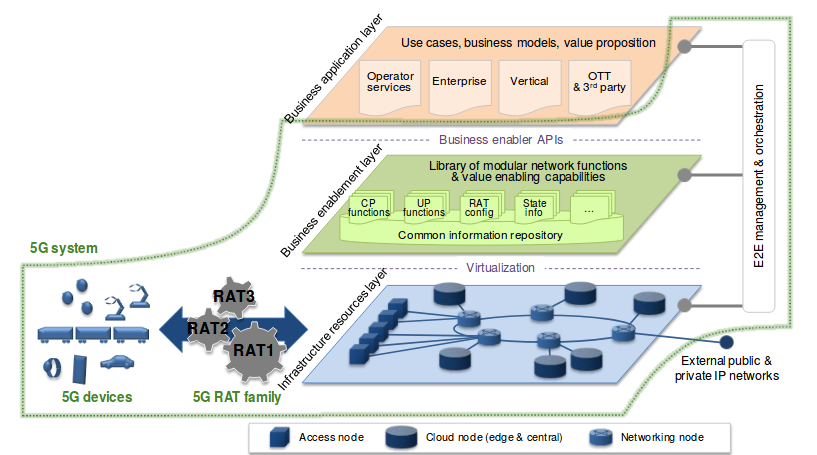
\includegraphics[scale=0.55]{5garchitecture}
  \caption[5G Architecture]{5G Architecture~\cite{alliance20155g}}
  \label{chap:background:img:5garchitecture}
\end{figure}

This separation in layers allows to easily manage multiple identities 
differently: an Internet Service Provider (ISP) could manage a multitude of 
physical infrastructures and have multiple business enablements dislocated 
along an entire continent for example, but it could decide to have only a 
single centralized business application deployment that manage all the other 
layers resources.

\subsubsection{Network slicing}
\label{chap:background:sec:5g:sub:ns}
The role of a \emph{network slice} in a 5G architecture is to specifically
handle the Control-plane of a particular service (e.g. smartphones traffic,
autonomous driving, massive IoT), deploying resources in a manner that assure
the required latency, security and reliability. While some very peculiar and
legacy service could require specific hardware, the common resources between
services could be shared in a virtualized way, providing auto-scaling
capabilities in services that are under heavy network pressure.

\section{The VIBeS project}
This thesis started as a part of the VIBES project~\cite{vibesesa}, whose main
requirement is to enhance the performance of end-to-end IP based that involves
satellite connections. To reach this goal, the project specifications suggest to
exploit the 5G incoming technology and use the NFV-MANO architecture to perform
first packets elaboration and performance improvement and finally TCP/IP
satellite chunk optimization with the Performance Enhancing Proxy (PEP). The
VIBES project proposed five technical requirements:
\begin{enumerate}
  \item Analysis of the applicability of current and new Internet protocols in
  the proposed VNF-PEP architecture
  \item Implementation of a VNF-PEP prototype
  \item Building of a PoC test platform
  \item VNF-PEP validation and performance tests on 5G use-cases
  \item Demonstration test-bed management
\end{enumerate}

\begin{figure}[t]
 \centering
 
\includegraphics[scale=1]{vibes_logo}
 \caption{ViBeS project logo}
 \label{chap:background:img:vibes_logo}
\end{figure}

\subsection{VNF-PEP architecture and internet protocols}
VNF-PEP is the softwarization of the usual PEP technology. One of the goals of
the project is to research and include this technology in the usual VNF
ecosystem to include without change satellite communications to the SFC. The
architecture of the systems will be based on clusters of containers whose
management and orchestration will follows the ETSI MANO architecture and SDN
principles. Thanks to VNF-PEP will be possible to dynamically take decisions on
how to optimize a certain communication.

%The analysis of this topic revealed to be trivial: since internet has many
%different protocols that would become infeasible to support all of them at the
%same time, packet encapsulation present itself as the only feasible solution:
%every packet incoming in the VNFs has already been encapsulated by a generic
%packet encapsulator/decapsulator,
%\todo{Also I think that the main purpose of UDP encapsulation is not to hide 
%the protocol used on the edges but 1) use a ``quick protocol to exchange data 
%among VNFs and 2) we are hiding the path not the protocol itself. As we were 
%discussing, we are creating some sort of proxy, so the aim will be the same 
%even if we support a plethora of protocols.''} making the whole architecture 
%independent from the protocol a particular flux of data. To achieve this, 
%several solutions have been studied, and at the end packet encapsulation with 
%TCP split (for TCP sessions) have been chosen. The rationale that guided us on 
%this choice is described in Chapter~\ref{chap:vnf_ns_impl}. \todo{Update 
%reference with the section of the explanation}
%
%\subsection{VNF-PEP prototype}
%
%Since the requirement for the whole system (MANO+PEP) were too challenging, the 
%goal shifted into creating a MANO test-bed and a working NFVI, excluding PEP. 
%The VNF architecture was shaped following the container orchestrator we decided 
%to use. An more detailed architectural implementation can be found at 
%Chapter~\ref{chap:archimpl}.
%
%\vspace{0.5cm}
%
%Starting with the first step of creating a MANO able to process incoming data
%packets through VNF functions, we encountered that many networking tools already
%present in the market required some tweaking and some integration, shifting our
%goal to create a complete European Telecommunications Standards Institutes
%(ETSI) Management and orchestrator (MANO) test-bed instead, following the
%specifications suggested in the RFC 7665, thus implementing only the first three
%requisites, without digging in the satellite data flow optimization. In
%particular, we discovered how, these tools, were suitable to create ETSI MANO
%and VNFs using virtual machine or exploiting cloud technologies, while they were
%not designed with enough flexibility an integration with Docker. In the next
%chapter we are going to take a deep analysis of the cited technologies 
%(Section~\ref{chap:prjan:sec:tech}, in order to provide to the reader enough 
%context to be able to understand our design choices we are going to describe 
%later.
%
%\noindent With this in mind, we performed a requirements analysis described in
%the next chapter.\todo{This should be put at the end of the introduction.}
% 

\section{Virtualization}
It is remarkable how cloud computing has surged in the recent years. This is due
the numerous features it carries, such as a great way to isolate processes and
mitigate possible attacks from malicious users. On top of that, it allows to run
virtual machines with different configurations, without bringing any changes to
the host machine. Indeed, the virtualization concepts refer to the property of
a machine to be virtualized. To achieve this, the components that forms a common
computer need to be virtualized too. Thus, these assets are recreated in this
virtualized manner, e.g. storage devices and computer network
resources~\cite{liu2014research}. At the time writing, there are two common
virtualization options: the virtualization through Hypervisor (defined also as
hypervisor-based) and the container virtualization.

\paragraph*{Hypervisor-based}
The first one is known for providing a very good isolation from the host
machine~\cite{eder2016hypervisor}, even if studies found possibilities for an
attacker to escape from the a virtual machine and operate on the host
one\footnote{An example can be found in
  \url{https://github.com/MorteNoir1/virtualbox_e1000_0day}}. Even though every
component in a hypervisor environment is virtualized, there are possibilities
for the ``guest'' OS (the virtualized one), to access to physical devices (like
USB keys attached on the ``host'' OS).

\paragraph*{Container-based}
Container-based virtualization uses a different approach to reach isolation.
Instead of creating a whole new stack, it applies very strict policies to the
programs running on the ``host'' machine. This concept has its roots back to the
jail environments, where group of process where isolated by the main OS, that
provided a virtualized file-system without any possibility to access to
different paths~\cite{canonico2007virtualization}. In this context, a
container-based application can be seen as a jailed application with policies
aimed to protect the host machine.

\begin{figure}[t]
  \centering
  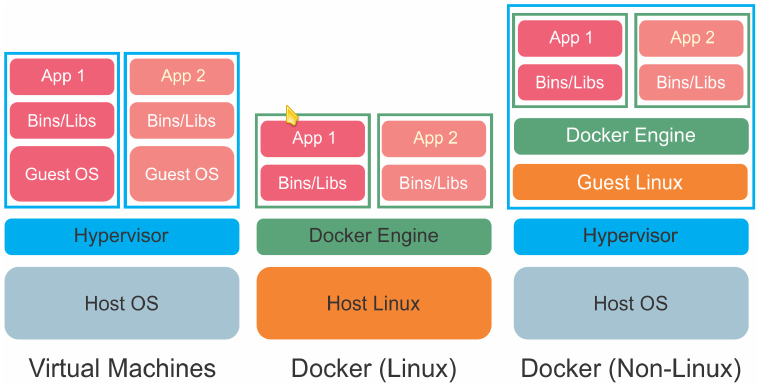
\includegraphics[scale=0.5]{docker_vs_hypervisor}
  \caption[Container-based emulation vs hypervisor emulation]{Container-based
    emulation, such as Docker vs hypervisor-based emulation~\cite{hung2016guidock}}
\end{figure}

\subsection{Network Virtualization}

Virtualization assumes another context when referred to networking: virtualized
networking allows multiple, heterogeneous networks to cohabit, increasing the
flexibility and manageability. This network separation creates two different
entities, that becomes decoupled: who provides the infrastructure (commonly
called InPs) and who provides the services (SPs). A virtual network can be
created aggregating one or more InPs, thus creating a virtual network end-to-end
service~\cite{chowdhury2009network}. An example of this are the Virtual Private
Networks (VPNs), that are able to cross public networks, giving access to
content that otherwise would not be available locally.

\section{Software-defined networking}
The concept of Software-defined networking (SDN) is not new: starting from
1996~\cite{sezer2013we} it aims to provide user-controlled management of data
forwarding in network nodes. This means to have the possibility to control the
forwarding procedures. A close examples of SDN implementations are Ethane and
OpenFlow, respectively created in 2007 and 2008. In an SDN architecture, there
is the decoupling of data and control plane (which will be explained in
Section~\ref{chap:background:sec:sdn:sub:cp}), but there is a centralization of
the networking logic and state~\cite{fundation2012software}. The use of an SDN
network is estimated to reduce the Capital Expenditure (CapEX) and Operational
Expenditure (OpEX) costs~\cite{benzekki2016software}.

\subsection{SDN stack}
\begin{figure}[ht]
 \centering
 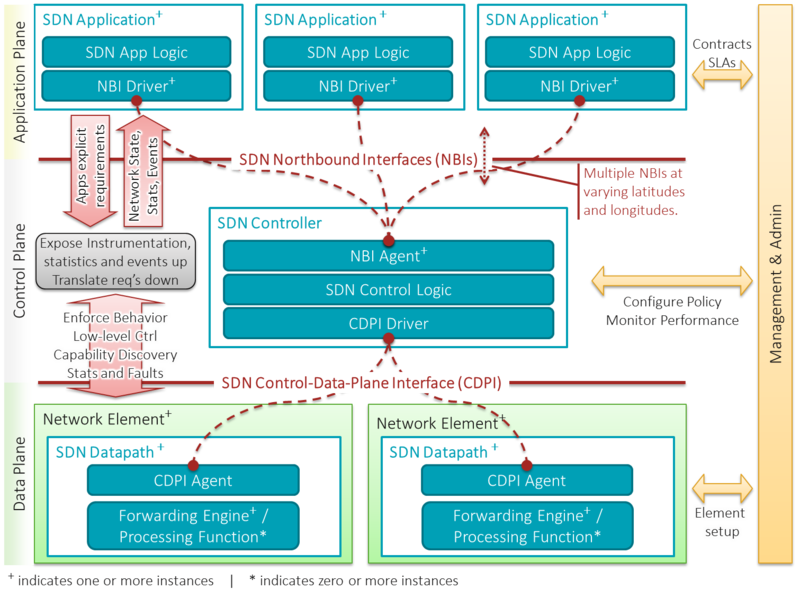
\includegraphics[scale=1.3]{sdn_architecture}
 \caption[SDN architecture schema]{SDN architecture schema. Is possible to 
denote the three layer logic: the Application plane, the Controller plane and 
the Data plane~\cite{fundation2013software}.}
 \label{chap:background:img:sdn_architecture}
\end{figure}

As the Figure~\ref{chap:background:img:sdn_architecture} illustrates, the SDN
architecture is formed by three layers, defined as planes, that accomplish
specific tasks~\cite{fundation2012software} as explained
in~\cite{fundation2013software}. Below we will perform a brief explanation of
each plane.

\subsubsection{Application plane}
In general, this layer is responsible of abstracting the SDN network control
management~\cite{benzekki2016software}. The application plane holds SDN
applications, programs that have the possibility to change the way the SDN
network forwards the data. These applications have the possibility to access
hardware capabilities through specific API, that are called \emph{northbound}
interfaces (NBI). These interfaces usually, acts like a bridge between the SDN
applications and the SDN controllers and are usually implemented in an open and
vendor-neutral way~\cite{fundation2013software}.

\subsubsection{Control plane}
\label{chap:background:sec:sdn:sub:cp}
The SDN controllers, as just said in the previously, receives requests from the
SDN applications. Since the controller is centralized, it can therefore exploit
the complete knowledge of the network. This gives the possibility to apply
networking optimization like flow management~\cite{sezer2013we}. The controller
abstracts from the network complexity, and it can collect information about the
network performing requests to the \emph{southbound} interfaces. The control
plane can have multiple controllers, that are in turn federated thanks to the
\emph{eastbound} and \emph{westbound} (e.g.
HyperFlow)~\cite{benzekki2016software} interfaces, that allow several existing
controller written even with different languages to coexists.

\subsubsection{Data Plane}
The data plane is the lowest plane and it provides the aforementioned
\emph{southbound} API. This API can be deployed in two different kind of
scenarios: for in-band communications and for out-of-band
communications~\cite{benzekki2016software}. The data plane gives access to the
physical and virtual switches, routers and access-points, and it gives the
possibility to perform programmatic forwarding operations, but it is also able
to provide statistic reporting and it supports event notifications.

\subsection{OpenFlow protocol}
OpenFlow is an open communication protocols that enables the possibility to
actually program networks, offering the possibility to change the flow-tables
for layer 3 switches and for routers~\cite{mckeown2008openflow}. In other words,
the OpenFlow protocol gives the possibility for controller to access at these
components. Routes can be changed based on the typology of the packet, or based
on the state of the network (i.e. if a network is under heavy load, certain
packages can be discarded).

\begin{figure}[t]
 \centering
 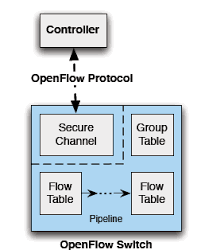
\includegraphics[scale=0.65]{openflow}
 \caption{OpenFlow protocol communication graph}
 \label{chap:background:img:openflow_protocol}
\end{figure}

In the Figure~\ref{chap:background:img:openflow_protocol} we have a schema of
what we said before: every switch has a flow table that gets updated thanks the
OpenFlow protocol by the SDN controller, that is the one managing the whole
network.

\section{Network slicing}
Internet Service Providers (ISP) provides networking services to a wide range of
users, that have different necessities between them, and that can require
different kind of characteristics, e.g. a network connectivity in a travelling
train has different networking requirements from the one deployed in a company.
It is with these presuppositions that emerges the necessity of service
optimization based on the users necessities. To solve this problem in the recent
years the concept of Networks Slice (NS) has been
introduced~\cite{alliance20155g}. The NS aims to logically separate this set of
services that present different use-cases, and in order to achieve this it
exploits the SDN and Network Function Chaining (NFC) that allows network
softwarization~\cite{ordonez2017network}.

\subsection{Network slice layers}

Even if the first idea of NS goes back to 2002~\cite{peterson2003blueprint}, NSs
ancestor can be found in VLANs, that allows different hosts with no physical
connectivity to be in the same network. The NS concept has attracted a lot of
interest especially from the Industries, that is trying to introduce them in the
5G mobile network standard. About this, more details are provided in
Section~\ref{chap:background:sec:5g:sub:ns}.

\begin{figure}[t]
  \centering
  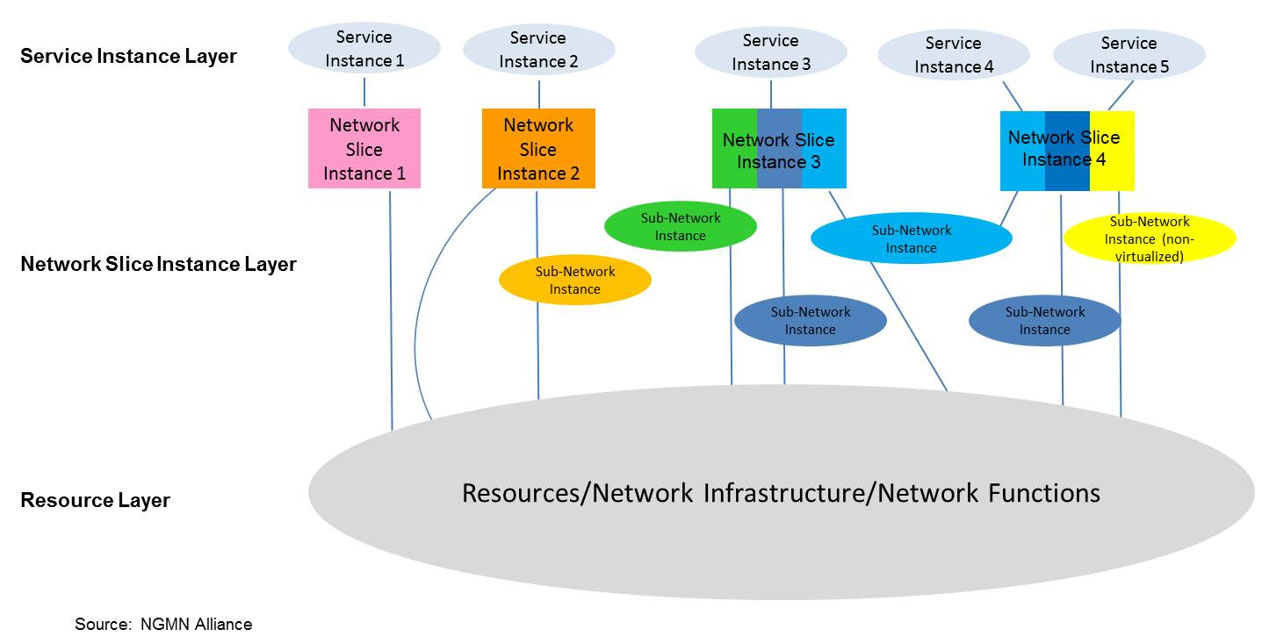
\includegraphics[scale=0.2]{networkslicing}
  \caption[The three layers model of network slicing]{The three layers model of
    network slicing~\cite{alliance2016description}}
  \label{chap:background:img:network_slicing}
\end{figure}

As is possible to see from the Figure~\ref{chap:background:img:network_slicing},
a network slice is divided in multiple layers, namely the Service Instance
Layer, the Network Slice Instance Layer and the Resource Layer.

\subsubsection{Service Instance Layer}
The first layer we presented, the \emph{Service Instance Layer}, represents the
business or user services supported. These services are achieved thanks to the
Network Functions (NF)~\cite{kotulski2017end}.

\subsubsection{Network Slice Instance Layer}
Instead, the \emph{Network Slice Instance Layer} as is possible to see it
contains multiple sub-network instances, that can be virtualized or
non-virtualized.

\paragraph*{Network Functions}
The concept behind NF is to usually elaborate incoming data and forward it to
destination. NFs can be physical of virtualized: in the first case is commonly a
set of hardware devices, in the second case instead it can be a software
implementation, decoupled from the hardware where its running. The Virtualized
Network Functions (VNFs), that are recently emerging propose a multitude of
challenges, especially regarding their latency, reliability and efficiency due
their virtualized nature of network function.

\vspace{0.5cm}

\noindent Every NF should be isolated, so that it only has the possibility to
consume a defined set of resources, otherwise the functions running on top of it
could suffer performance degradation~\cite{richart2016resource}. Isolation has
the benefits of offering more security and the possibility to individually
manage the slice~\cite{ordonez2017network}. Slices have to respond to a defined
set o requisites, first of all the possibility to being created by a template,
defined as Network Slice Template (NST). After the NS and the related resources
are created, a NS should be activated. Obviously, for a NS there should be the
possibility to bring changes on-the-fly, and to decommission or deactivate it,
freeing all the occupied resources~\cite{slice20183gpp}.

\subsubsection{Resource Layer}
This layer contains all the physical and virtualized resources, that are needed
to the network slice to properly function. The resources are divided in
computational and storage resources.

\subsection{Network Function Virtualization}
Concept recently developed in 2012 by the ETSI organization, the Network
Function Virtualization (NFV), is a network architecture concept that aims, with
the virtualization technologies available in the market, to virtualize network
nodes. It is believed that NFV will transform the way the global communications
will work, thanks to its disruptive trend in the networking
industry~\cite{gray2016network}. Essentially, a NFV, working in harmony with the
NS aims to provide sufficient packet processing efficiency, especially in
environments such as the cloud one.

\begin{figure}[t]
  \centering
  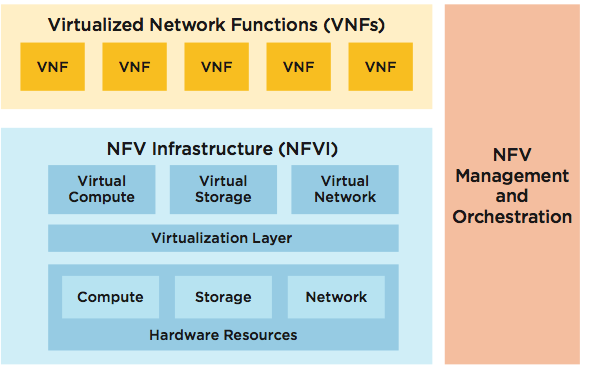
\includegraphics[scale=2]{etsi_arch}
  \caption[Network Function Virtualization reference architecture]{Network
    Function Virtualization reference architecture~\cite{etsi2013gs}}
  \label{chap:background:img:etsi_arch}
\end{figure}

\noindent The NFV has its own architecture, divided in three main components:
\begin{description}
\item[Virtualized Network Function] that is a software implementation able to fun
  a network function over a NFVI;
\item[NFVI Infrastructure (NFVI)] that includes different physical resources
  and their respective virtualization, that have to support the execution of the
  aforementioned VNFs;
\item[NFV Management and Orchestrator] that has the main role to orchestrate the
  lifecycle of the available resources and of the network functions running on
  top of them.
\end{description}

In the next section we are going to dig a little bit about the component that
have not been explained yet.

\subsubsection{Network Function Virtualized Infrastructure}
With the term NFVI we mean the totality of all the hardware and software
components where NFVs run~\cite{etsi2013gs}. The NFVI does not have to be
centralized, but it can span across multiple locations, even though the
resources should be virtualized in a manner from the VNF point of view that they
look like coming form a single entity. The computing hardware that composes the
NFVI can be either Commercial-of-the-shelf (COTS) hardware or a specialized one,
while for the storage there is the possibility to have a Network Attached
Storage (NAS) o a ``local'' storage directly on the server~\cite{etsi2013gs}.
Finally, network resources, composed by switches, routers and links (both wired
and wireless) can span between different domain, that can be of two typologies:
\begin{itemize}
\item NFVI-PoP
\item Transport network
\end{itemize}

\subsubsection{NFV MANagement and Orchestration}

\begin{figure}[t]
  \centering
  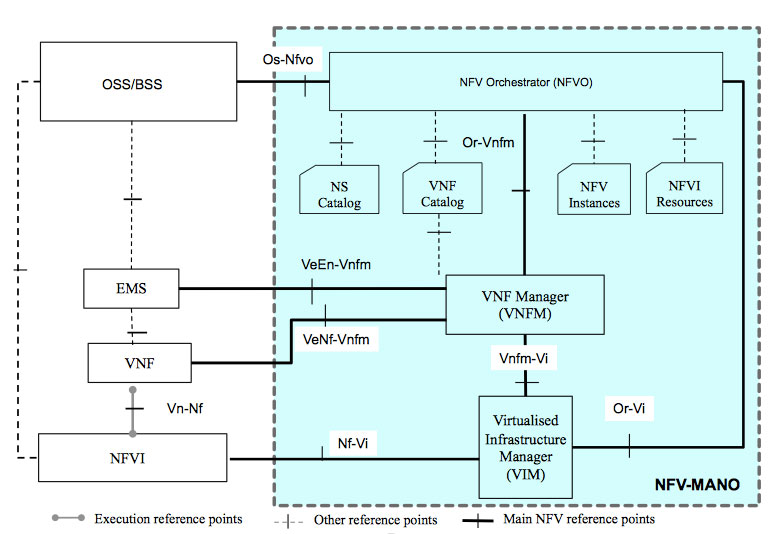
\includegraphics[scale=0.7]{etsimano}
  \caption[ETSI NFV MANO framework]{ETSI NFV MANO
    framework~\cite{mijumbi2016management}}
  \label{chap:background:img:etsimano}
\end{figure}

The MANagement and Orchestration (MANO) architecture is divided in turn in three
main components, such as the Virtual Infrastructure Manager (VIM), the VNF
Manager (VNFM) and the NFV Orchestrator (NFVO). The MANO organize and holds
important data, regarding the Network Service (NS) catalog, the list of the VNFs
definitions (VNF catalog) and the current NFV instances and the NFVI resources.

It is important to note how the mano is a critical aspect in ensuring
cooperation between the NFVI and the VNFs. On top of that, is able to provide
and manage the VNFs lifecycle~\cite{mijumbi2016management}.

\paragraph{VIM}
As we can see from the Figure~\ref{chap:background:img:etsimano}, it is possible
to denote the position of this component in the schema. The VIM has the role to
communicate with the NFV infrastructure, and to control its physical and virtual
resources. A VIM should has the possibility to control one or more of NFVI. In
general a VIM can be in charge of control a defined set of
NFVI~\cite{mijumbi2016management}

\paragraph{VNFM}
The VNFM, as we can see from the schema, interacts with the Data repositories,
the NFVO and with the VNFs. Its role is to manage the lifecycle of VNFs. The
VNFM can handle one or multiple VNF instances.

\paragraph{NFVO}
We can see how the NFVO is the component with the most connections in the whole
architecture, and its able to interact with the OSS/BSS, the data repositories,
the VNFM and the VIM. The aim of the NFVO is thus to orchestrate both the
resources and the services.

\paragraph{Data Repositories}
Data repositories can be seen as a sort of databases, holding information about
the VNF definitions, the VNF instances with the respective lifecycle status, and
list of the Network Services defined and the resources available and occupied of
the NFVI.

\section{Service Function Chaining (SFC)}
Another important component we have to talk about is the SFC, defined as a
concept that it collocates logically above the NFVs. As said in~\cite{rfc7665}:
\begin{displayquote}
The definition and instantiation of an ordered set of service functions and
subsequent ``steering'' of traffic through them is termed Service Function
Chaining (SFC).
\end{displayquote}

\paragraph*{Service Function}
A single element of an SFC is called Service Function (SF), and its duty is to
elaborate the packets incoming and to forward them to the next receiver. SFs, as
for NFs, can be virtualized or be a set of hardware functions. SF does not
necessary know its part of a chain, and this defines it as SFC unaware or, on
the contrary, SFC aware.

\paragraph*{Architectural view}
About the architectural view of SFCs, proposal defines several assumptions on
them, starting from considering every element of the chain an opaque processing
unit. Another important assumption is that there is no global or standard SF
chaining logic~\cite{rfc7665}. SFC can be easily seen as a graph, because some
SF can have multiple address to forward the elaborated data, thus creating what
is defined as \emph{fork} that ends up forming different branches. This could
lead to loops, that must be treated consequently.

\paragraph*{Forwarding strategies}
At high level, SFC proposes an abstracted view of a service, with a defined set
of required SFs that must be executed in a particular order. These services can
be unidirectional if they support data coming only from one direction, thus
following the chain from the first SF to the last one, or they can be
bidirectional, when they supports data coming from both directions, and thus the
first SF can be the last one~\cite{rfc7665}. The forwarding logic has to be
managed by the Service Function Forwarder (SFF), that forwards the data
following the Service Function Path (SFP) defined.

\paragraph*{Data encapsulation}
The data passing inside an SFC must be encapsulated to ensure its integrity.
Data encapsulation enables the possibility of sharing metadata/content, and to
share information about the SFP to follow. Data gets continuously encapsulated
and decapsulated between SFs, to give them the possibility to elaborate the
payload contained.

\subparagraph*{Network Service Header (NSH)}
The encapsulation has an header that is well defined and described in detail
in~\cite{rfc8300}. This header is composed by a 4-byte base header, and a 4-byte
Service Path Header (SPH). The base header provides information about the services
header and the kind of protocol contained as the payload, while the service path
header provides path identification and location within a define Service Path
(SP). Finally, the Context Header carries metadata.

To further digging in the rabbit hole, the base header has several fields,
identifying the NSH version, the total Time To Live (TTL) of a packet, the
length of it, an additional metadata field and at the end it has a field to
identify the protocol of the encapsulated data.

The SPH contains the 24-bit Service Path Identifier (SPI) and a Service Index
(SI), that provides the location within the SFP.

\subparagraph*{Context header}
There are two kind of context header definitions: one with a fixed context
header length (16-Byte) and one with a dynamic context header length.

\noindent Regarding this field, the standard does not make any assumption about
the content, and it is left free to be filled with custom metadata. The only
requirement is to set this filed with zeroes when is not used.

\begin{figure}[t]
  \centering
  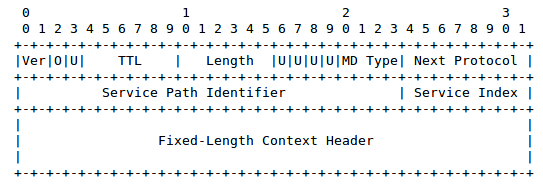
\includegraphics[scale=0.6]{nshtype1}
  \caption[NSH MD Type \texttt{0x1}]{NSH MD Type \texttt{0x1}~\cite{rfc8300}.
    The context header in this NSH has a fixed length. There is another possible
    context header that has a variable length.}
  \label{chap:background:img:nshtype1}
\end{figure}
